\documentclass[aspectratio=169,xcolor=dvipsnames]{beamer}
\usetheme{Berlin}

\usepackage[english]{babel} % Cambiado a español para acentos y textos automáticos
\usepackage{hyperref}
\usepackage{graphicx}
\usepackage{booktabs}
\usepackage{amsmath}
\usepackage{lettrine}
\setbeamertemplate{caption}[numbered]
\usepackage[dvipsnames,svgnames,x11names]{xcolor}
\usepackage{xurl}
\usepackage{hyperref}
\usepackage{algorithm}
\usepackage{algorithmicx}
\usepackage{algpseudocode}
\usepackage{adjustbox}
\hypersetup{
    colorlinks=true,
    linkcolor=cyan, % Color más visible en temas oscuros
    filecolor=blue,
    urlcolor=blue,
    citecolor=blue,
}
%----------------------------------------------------------------------------------------
\usepackage{listings}
\usepackage{xcolor}

\definecolor{codegreen}{rgb}{0,0.6,0}
\definecolor{codegray}{rgb}{0.5,0.5,0.5}
\definecolor{codepurple}{rgb}{0.58,0,0.82}
\definecolor{backcolour}{rgb}{0.97,0.97,0.99}

\lstdefinestyle{MATLABStyle}{
  language=Matlab,
  basicstyle=\ttfamily\footnotesize,
  keywordstyle=\color{blue}\bfseries,
  commentstyle=\color{codegreen},
  stringstyle=\color{violet},
  numberstyle=\tiny\color{gray},
  breakatwhitespace=false,
  breaklines=true,
  captionpos=b,
  keepspaces=true,
  numbers=left,
  numbersep=5pt,
  showspaces=false,
  showstringspaces=false,
  showtabs=false,
  tabsize=2,
  frame=lines,
  framerule=0.4pt,
  backgroundcolor=\color{backcolour}
}
\lstset{style=MATLABStyle}

%----------------------------------------------------------------------------------------
%	TITLE PAGE
%----------------------------------------------------------------------------------------


%----------------------------------------------------------------------------------------
%	TITLE PAGE
%----------------------------------------------------------------------------------------

\title{Artificial Neural Networks}
\subtitle{Chapter 3: Supervised Learning Neural Networks \\ Neural Network Types}

\author{Prof. Dr. BARSEKH-ONJI Aboud}

\institute
{
    Facultad de Ingeniería \\
    Universidad Anáhuac México
}
\date{\today}

%----------------------------------------------------------------------------------------
%	PRESENTATION SLIDES
%----------------------------------------------------------------------------------------

\AtBeginSection[]
{
  \begin{frame}{Agenda}
    \tableofcontents[currentsection]
  \end{frame}
}

\begin{document}

\begin{frame}
    \titlepage
\end{frame}

%------------------------------------------------
\section{Introduction}
%------------------------------------------------

\begin{frame}{Neural Network Architectures}
    \begin{block}{Architectural Classification}
    Neural Networks are characterized by:
    \begin{itemize}
        \item \textbf{Architecture}: The arrangement of neurons and their connections.
        \item \textbf{Learning Algorithm}: The method used to adjust weights.
        \item \textbf{Activation Functions}: The equations controlling the output.
    \end{itemize}
    \end{block}
    
    This chapter focuses on the main architecture types for Supervised Learning:
    \begin{itemize}
        \item Feedforward Neural Networks (FNN)
        \item Recurrent Neural Networks (RNN)
    \end{itemize}
\end{frame}

%------------------------------------------------
\section{Feedforward Neural Networks}
%------------------------------------------------

\begin{frame}{Feedforward Classification}
    \begin{block}{Characteristics}
    In Feedforward Neural Networks (FNN), the signal flows in only one direction: from input to output. There are no cycles or loops.
    \end{block}
    
    \begin{itemize}
        \item Single-Layer Perceptron
        \item Multi-Layer Perceptron (MLP)
        \item Functional Link Neural Networks (FLNN)
        \item Product Unit Neural Networks (PUNN)
    \end{itemize}
\end{frame}

\begin{frame}{Single-Layer Perceptron}
    \begin{columns}[t]
        \column{.48\textwidth}
            \begin{block}{Structure}
            The simplest form of ANN.
            \begin{itemize}
                \item Only has Input and Output layers.
                \item Can only solve linearly separable problems.
                \item Uses step activation function (originally).
            \end{itemize}
            \end{block}
        \column{.48\textwidth}
            % Placeholder for figure
            \begin{figure}
                \centering
                \includegraphics[width=0.8\textwidth]{Figures/singlelayer.png}
                \caption{Single-Layer Network Structure.}
            \end{figure}
    \end{columns}
\end{frame}

\begin{frame}{Multi-Layer Perceptron (MLP)}
            \begin{alertblock}{Adding Hidden Layers}
            Includes one or more "hidden" layers between input and output.
            \begin{itemize}
                \item Can approximate any continuous function (Universal Approximation Theorem).
                \item Solves non-linearly separable problems (e.g., XOR).
                \item Typically trained with Backpropagation.
            \end{itemize}
            \end{alertblock}
            % Placeholder for figure
           
\end{frame}

\begin{frame}{Multi-Layer Perceptron (MLP)}
 \begin{figure}
                \centering
                \includegraphics[width=0.65\textwidth]{Figures/FFNN.png}
                \caption{Multi-Layer Network Structure.}
            \end{figure}
\end{frame}

\begin{frame}{Functional Link Neural Networks (FLNN)}
    \begin{block}{Higher-Order Combinations}
    Instead of adding hidden layers, inputs are expanded using functional links.
    \end{block}
    
    \begin{itemize}
        \item \textbf{Tensor Model}: Multiplies inputs ($z_1 z_2, z_1^2$, etc.)
        \item \textbf{Functional Expansion}: Passing inputs through functions ($\sin(z_1), \cos(z_1)$).
    \end{itemize}
    
    Advantages: Faster training (no hidden layers to train), effectively a single-layer network with expanded input space.
\end{frame}

\begin{frame}{Functional Link Neural Networks (FLNN)}
 \begin{figure}
                \centering
                \includegraphics[width=0.65\textwidth]{Figures/FLNN.png}
                \caption{Multi-Layer Network Structure.}
            \end{figure}
\end{frame}

\begin{frame}{Product Unit Neural Networks}
    \begin{block}{Multiplicative Inputs}
    Instead of summing weighted inputs ($\sum z_i v_i$), Product Units calculate the weighted product:
    \begin{equation}
        net_j = \prod_{i=1}^{I} z_i^{v_{ji}}
    \end{equation}
    \end{block}
    \begin{itemize}
        \item Can implement higher-order functions more efficiently.
        \item Harder to train (complex error surfaces).
    \end{itemize}
\end{frame}

%------------------------------------------------
\section{Recurrent Neural Networks}
%------------------------------------------------

\begin{frame}{Recurrent Features}
    \begin{alertblock}{Feedback Loops}
    Recurrent Neural Networks (RNNs) have feedback connections where outputs are fed back into their own inputs or previous layers.
    \end{alertblock}
    
    \begin{itemize}
        \item **Memory**: They have a temporal state/memory of previous inputs.
        \item Suitable for time-series prediction and sequence processing.
    \end{itemize}
\end{frame}

\begin{frame}{Elman Recurrent Network}
            \begin{block}{Context Layer}
            A simple recurrent network (SRN).
            \begin{itemize}
                \item Hidden layer outputs are copied to "Context Units".
                \item Context units feed back into the hidden layer in the next time step.
                \item Allows learning of temporal patterns.
            \end{itemize}
            \end{block}
            % Placeholder for figure
            
\end{frame}


\begin{frame}{Jordan Recurrent Network}
    \begin{block}{Output Feedback}
    Similar to Elman, but the feedback comes from the \textbf{Output Layer} instead of the hidden layer.
    \end{block}
    
    \begin{itemize}
        \item Context units store the previous output.
        \item Often used for control systems where the next state depends on the previous action (output).
    \end{itemize}
\end{frame}


\begin{frame}{Elman and Jordan Recurrent Network}
    \begin{columns}[t]
        \column{.5\textwidth}
        \begin{figure}
                \centering
                \includegraphics[width=0.8\textwidth]{Figures/elman.png}
                \caption{Elman Recurrent Network Structure.}
            \end{figure}
        \column{.5\textwidth}
        \begin{figure}
                \centering
                \includegraphics[width=0.8\textwidth]{Figures/Jordan.png}
                \caption{Jordan Recurrent Network Structure.}
            \end{figure}
            \end{columns}
\end{frame}

\section{Time-Delay Neural Networks}
\begin{frame}{Time-Delay Neural Networks}
        \begin{block}{The output of a TDNN is calculated as:}
            \begin{equation}
o_{k,p} = f_{o_k} \left( \sum_{i=1}^{I+1} u_{ki}z_i + \sum_{j=1}^{J} w_{kj}f_{y_j} \left( \sum_{i=1}^{I+1} v_{ji}z_i + \sum_{l=1}^{j-1} s_{jl}y_l \right) \right)
\end{equation}
        \end{block}
\end{frame}
\begin{frame}{Time-Delay Neural Networks}

        \begin{figure}
                \centering
                \includegraphics[width=0.4\textwidth]{Figures/TDNN.png}
                \caption{Time-Delay Neural Network Structure.}
            \end{figure}
\end{frame}


\section{Cascade Neural Networks}
\begin{frame}{Cascade Neural Networks}
        \begin{block}{The output of a Cascade Neural Network is calculated as:}
            \begin{equation}
o_{k,p} = f_{o_k} \left( \sum_{j=1}^{J+1} w_{kj}f_{y_j} \left( \sum_{i=1}^{I} \sum_{t=0}^{n_t} v_{j,i(t)}z_{i,p}(t) + z_{I+1}v_{j,I+1} \right) \right)
\end{equation}
        \end{block}
\end{frame}
\begin{frame}{Cascade Neural Networks}
        \begin{figure}
                \centering
                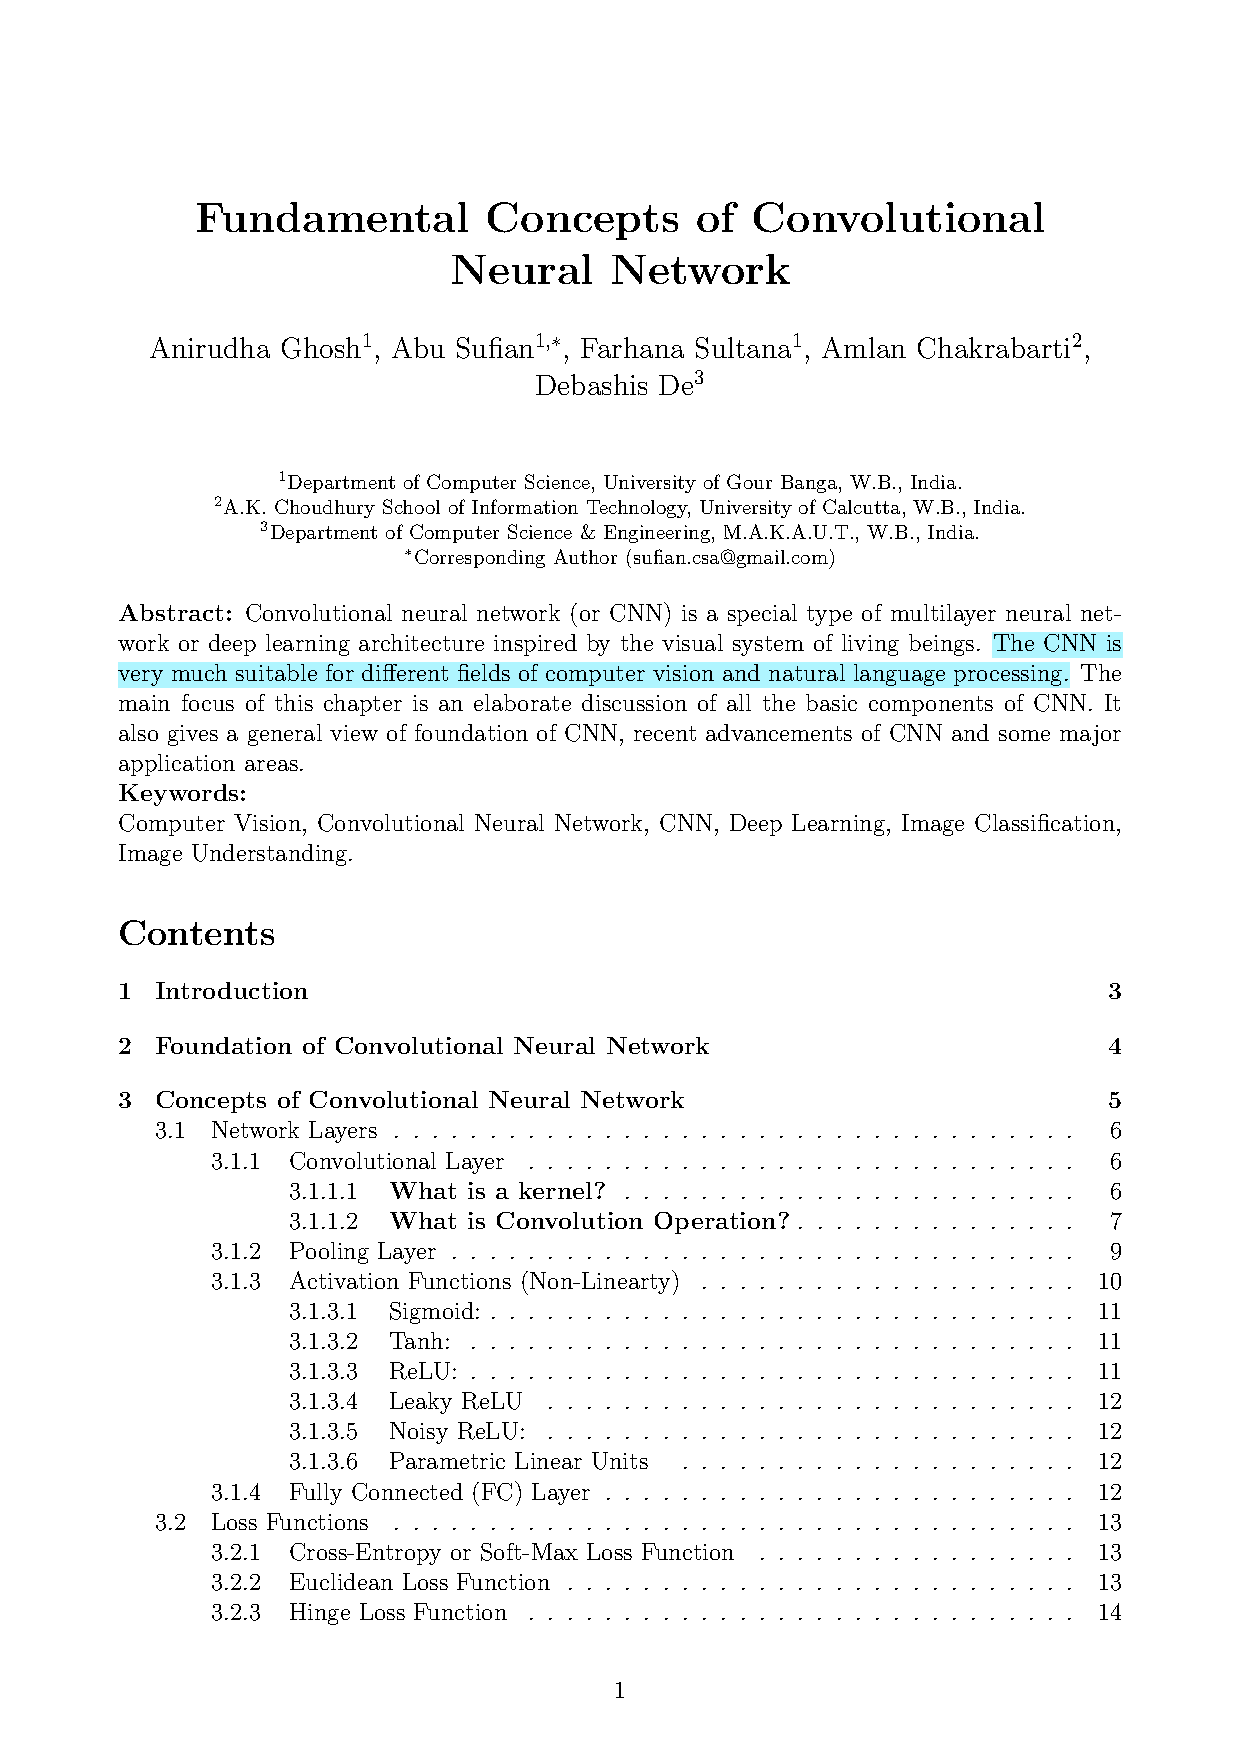
\includegraphics[width=0.5\textwidth]{Figures/CNN.png}
                \caption{Cascade Neural Network Structure.}
            \end{figure}
\end{frame}
%------------------------------------------------
\section{Conclusion}
%------------------------------------------------

\begin{frame}{Summary}
    \begin{itemize}
        \item \textbf{Feedforward Networks} (MLP) are the standard for static pattern classification and regression.
        \item \textbf{Functional Link} and \textbf{Product Units} offer alternative ways to handle non-linearity without deep layers.
        \item \textbf{Recurrent Networks} (Elman, Jordan) introduce memory, making them essential for temporal and sequential data problems.
        \item \textbf{Time-Delay Neural Networks} are used for time series prediction and sequence processing.
        \item \textbf{Cascade Neural Networks} are used for function approximation and regression.
    \end{itemize}
\end{frame}

\end{document}
